\documentclass[UTF8, twoside, titlepage]{ctexart}

\usepackage[a4paper]{geometry}
\geometry{hmarginratio=1:1}
\geometry{bottom=4cm}

\setlength{\parskip}{0.5\baselineskip}

\usepackage{hyperref}
\usepackage{fancyhdr}
\pagestyle{fancy}
\usepackage{emptypage}
\usepackage{multicol}

\usepackage{algorithm}
\usepackage{algorithmic}
\renewcommand{\algorithmicrequire}{\textbf{Input:}} \renewcommand{\algorithmicensure}{\textbf{Output:}}
\renewcommand{\algorithmicprint}{\textbf{output}}

\newenvironment{lex}
{
	\linespread{1.2}
	\leftskip=2.5cm
	\rightskip=2.5cm
	\itshape
	\setlength{\parindent}{-1cm}
}
{\par}

\usepackage{listings}
\usepackage[dvipsnames]{xcolor}
\lstset{
	basicstyle=\ttfamily,
	keywordstyle=\color{blue},
	commentstyle=\color{OliveGreen},
	stringstyle=\color{RawSienna}, 
	tabsize=4,
	columns=flexible,
	xleftmargin=1.4cm,
	xrightmargin=1.4cm,
	showspaces=false,
	showstringspaces=false,
	showtabs=false,
	breaklines=true,
	breakatwhitespace=false,
}

\begin{document}
\songti
\zihao{-4}

\begin{titlepage}
	\centering
	\vspace*{0.6in}
	\begin{figure}[h]
		\centering
		
\includegraphics[width=8cm]{images/bit-logo.png}
	\end{figure}
	\vspace{0.9in}
	{\heiti \zihao{0} 词法分析器实验}
	\vspace{\fill}
	\begin{table}[h]
		\centering
		\zihao{4}
		\begin{tabular}{rl}
			姓 \ 名: & 徐恒达 \\
			学 \ 号: & 1120151811 \\
			班 \ 级: & 07111504
		\end{tabular}
	\end{table}
	\vspace{0.4in}
\end{titlepage}
\cleardoublepage

\pagenumbering{Roman}
\tableofcontents
\cleardoublepage

\pagenumbering{arabic}

\section{实验目的}
利用高级语言设计并实现一个词法分析程序,加深对词法分析原理的理解。并在实验中掌握扫描器的工作原理,以及对输入的程序设计语言源代码进行扫描过程中将其分解为各类不同属性的单词的词法分析方法。

\section{实验内容}
以C语言作为源语言,构建C语言的词法分析器,对于给定的测试程序,输出XML格式的属性字符流。词法分析器的构建按照C语言的词法规则进行。

\section{实验过程}
本次实验中的C语言词法分析器基于现行的ISO C11标准(ISO/IEC 9899:2011 Programming languages C)。标准中将C语言中的词法元素分为5类,分别是关键字(keyword)、标识符(identifier)、常量(constant)、字符串字面量(string literal)和分隔符(punctuator),本次实验也严格按这5类进行识别,唯一的不同就是实验中把ISO标准中的分隔符进一步分为了限界符(delimiter)和运算符(operator),限界符包含了只有分隔作用没有运算作用的6个符号(,),[,],\{,\},.,->,其余符号均识别位运算符,以方便后续的处理。

本次实验中的词法分析器几乎实现了ISO C11标准中词法元素的全集,只有通用字符名(universal character name)和多字节字符(multibyte character)这两类使用频率非常低的词法元素没有进行识别,其余所有的符合ISO C11定义的词法元素均能有效识别,并且有健全的出错处理机制,准确划分出非法单词的范围,不会因为某个非法单词而导致其后的识别过程发生混乱。

实验中对ISO标准中的5类单词重新进行了一些划分,使总的识别任务分为几个任务量均不太大的子任务。将标识符和关键字的识别放在一起,因为关键字本身就是符合标识符定义的特殊单词;因为常量包含的单词范围很大,规则各异,故将常量的识别分为整型常量、浮点型常量和字符常量的识别,但识别后均标注为常量类型;最后是把分隔符分为了限界符和运算符,识别之后仍分别标注限界符和运算符。在词法分析器输出的属性字流中共有7种类型,分别是关键字(keyword)、标识符(identifier)、常量(constant),字符串(string),限界符(delimiter),运算符(operator)和非法(illegal)。词法分析器的设计和实现也针对这7种类型展开。

对于每一种要识别的单词,首先根据ISO C11标准中给出的词法定义写出其对应的正规式,然后将正规式转化为等价的DFA,最终将每一类单词的DFA和并在一起并用程序实现。本次实验中采用Java语言以面向程序的方法实现自动机,即对自动机中的每一个状态定义一个决定其后继状态的状态转换函数。如图\ref{fig:flow}所示。

\begin{figure}[htbp]
	\centering
	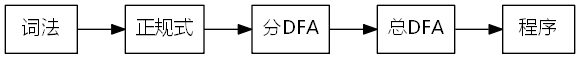
\includegraphics[width=12cm]{images/flow.png}
	\caption{词法分析器实现流程}
	\label{fig:flow}
\end{figure}

\subsection{标识符和关键字}
ISO C11标准中对于标识符和关键字的词法定义如下。

\begin{lex}
identifer:\\
	nondigit\\
    identifer nondigit\\
    identifer digit
    
nondigit: \normalfont{one of}\\
{
	\normalfont
	\ttfamily
	\_\\
	a b c d e f g h i j k l m n\\
	o p q r s t u v w x y z\\
	A B C D E F G H I J K L M N\\
	O P Q R S T U V W X Y Z	
}

\itshape
digit: \normalfont{one of}\\
{
	\normalfont
	\ttfamily
	0 1 2 3 4 5 6 7 8 9
}

\itshape
keyword: \normalfont{one of}\\
{
	\normalfont
	\ttfamily
	auto break case char const continue default do\\
    double else enum extern float for gotoif inline\\
    int long register restrict return short signed\\
    sizeof static struct switch typedef union\\
    unsigned void volatile while \_Alignas \_Alignof\\
    \_Atomic \_Bool \_Complex \_Generic \_Imaginary\\
    \_Noreturn \_Static\_assert \_Thread\_local
}
\end{lex}

标识符的定义简而言之就是由字母、数字和下划线组成且开头不能为数字的单词。转化为等价的正规式如下。

\begin{lstlisting}
identifer = (letter|_) (letter|digit|_)*
letter = [0-9]
digit = [a-zA-Z]
\end{lstlisting}

关键字完全符合标识符的定义,可以理解为是标识符的特例。在实际识别过程中不需要对关键字设置单独的识别规则,在识别出标识符后,判断如果是关键字集合中的元素就标记为关键字,否则标记为标识符。

识别标识符的DFA如图\ref{fig:identifier}所示。

\begin{figure}[htbp]
	\centering
	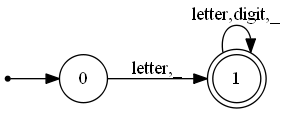
\includegraphics[scale=0.54]{images/identifier.png}
	\caption{识别标识符的DFA}
	\label{fig:identifier}
\end{figure}

在实际编程中,程序处在1状态后,并不知道此时应该直接识别单词还是继续等待下一个字符,只有当读入一个不是字母数字和下划线的字符后,程序才会知道到当前字符的前一个字符为止是一个完整的标识符。因此在程序中1状态并不是一个接受态,而从1状态读入一个其他字符后进入的状态才是真正的接受态。要到达此状态后,程序将当前字符之前的单词识别为标识符,并将当前字符放回缓冲区,重新回到0状态开始下一轮的识别。实际上在识别过程中大部分单词都像这样需要一个额外的字符才能确定识别。为了突出问题核心,此处以及下文中并没有将实际的接受态画出,但会对每个接受态进行说明。

\subsection{整数常量}
ISO C11中的常量分为整数常量、浮点数常量、字符串常量、枚举常量和字符常量。其中枚举常量就是标识符,这里不再单独处理,下面分别对其余4种进行识别。首先识别整数常量。

整数常量分为十进制整数常量、八进制整数常量和十六进制整数常量,每一种都可以有整数后缀或者没有。

\begin{lex}
integer-constant:\\
	decimal-constant \\
	octal-constant \\
	hexconstant \\
	decimal-constant integer-suffix \\
	octal-constant integer-suffix \\
	hex-constant integer-suffix
\end{lex}

首先讨论不带整数后缀的常量。十进制整数常量的定义如下所示。

\begin{lex}
decimal-constant:\\
	nonzero-digit \\
	decimal-constant digit

digit: \normalfont{one of}\\
{
	\normalfont
	\ttfamily
	0 1 2 3 4 5 6 7 8 9
}

\itshape
nonzero-digit: \normalfont{one of}\\
{
	\normalfont
	\ttfamily
	1 2 3 4 5 6 7 8 9
}
\end{lex}

用文字描述可以为“以1到9之间的数字开头,其后可以跟任意数字”。用正规式描述如下,其中*表示符号可以出现零次或多次,?表示可以出现零次或一次。

\begin{lstlisting}
decimal-constant= nonzero-digit digit* integer-suffix?
\end{lstlisting}

八进制整数常量的定义如下所示。

\begin{lex}
octal-constant:\\
{
	{\normalfont \ttfamily 0} \\ 
	octal-constant octal-digit
}

\itshape
octal-digit: \normalfont{one of}\\
{
	\normalfont
	\ttfamily
	0 1 2 3 4 5 6 7
}
\end{lex}

用文字描述可以为“必须以0开头,其后可以跟0到7之间的任意数字”。正规式描述如下。

\begin{lstlisting}
octal-constant = 0 octal-digit* integer-suffix?
\end{lstlisting}

十六进制整数常量如下所示。

\begin{lex}
hex-constant:\\
	hex-prefix hex-digit \\
	hex-constant hex-digit
	
hex-prefix: \normalfont{one of}\\
{
	\normalfont
	\ttfamily
	0x 0X
}

\itshape
hex-digit: \normalfont{one of}\\
{
	\normalfont
	\ttfamily
	0 1 2 3 4 5 6 7 8 9\\
	a b c d e f\\
	A B C D E F
}
\end{lex}

用文字描述可以为“以前缀0x或0X开头,至少有一位十六进制数字”。 正规式描述如下。

\begin{lstlisting}
hex-constant = 0(x|X) hex-digit+ integer-suffix?
\end{lstlisting}

值得注意的是十进制和八进制常量开头的标志性数字也是其值的一部分,所以后面的数字可以有一个或多个,正规式中表现为数字后面加*,而十六进制的前缀标识0x并不作为其值的一部分,所以要求后面至少有一位十六进制数字,在正规式中表现为数字后面带+。

不带后缀的三种常量全部讨论完毕了,将这三类常量的正规式转化为等价的DFA如图\ref{fig:integer}所示。其中状态2表示识别整型常量,状态3表示识别八进制常量,状态13表示十六进制常量。这三个接受状态再编程时均需要再读入一个额外字符后才能结束识别。

\begin{figure}[htbp]
	\centering
	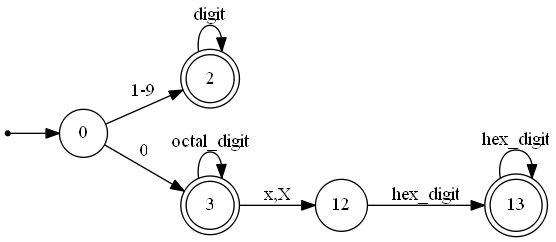
\includegraphics[scale=0.54]{images/integer.png}
	\caption{识别整数常量的DFA}
	\label{fig:integer}
\end{figure}

最后讨论整数后缀。定义如下。

\begin{lex}
integer-suffix:\\
	unsigned-suffix \\
	unsigned-suffix long-suffix \\
	unsigned-suffix long-long-suffix \\
	long-suffix \\
	long-suffix unsigned-suffix \\
	long-long-suffix \\
	long-long-suffix unsigned-suffix
	
unsigned-suffix: \normalfont{one of}\\
{
	\normalfont
	\ttfamily
	u | U
}

\itshape
long-suffix: \normalfont{one of}\\
{
	\normalfont
	\ttfamily
	l | L
}

\itshape
long-long-suffix: \normalfont{one of}\\
{
	\normalfont
	\ttfamily
	ll | LL
}
\end{lex}

从形式上看略有复杂,概括起来,后缀分为两部分,一部分是u,另一部分是l或ll,大小写均可。两部分可以只取一种,也可以全有,而且没有顺序限制。可以看出灵活性很大。用正规式描述如下。

\begin{lstlisting}
integer-suffix = 
	(u|U) |
	(u|U) (l|L|ll|LL) |
	(l|L|ll|LL) |
	(l|L|ll|LL) (u|U)
\end{lstlisting}

转化为等价DFA如图\ref{fig:int_suffix}所示。图中第一个状态x可以是图中的状态2、3或13,即完整的DFA中状态2、3和13之后都要接一个图中的自动机。自动机中每个状态都是接受态,因为后缀可以在任何一个位置停止。每一个接受态都是再读到一个额外字符后完成判断。

\begin{figure}[htbp]
	\centering
	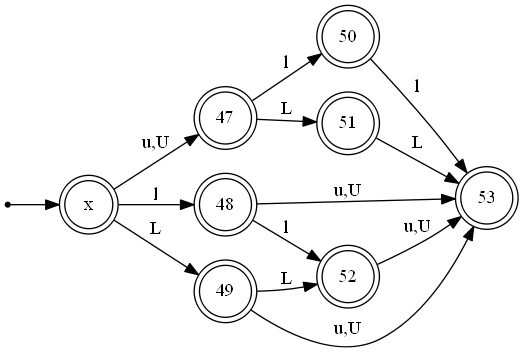
\includegraphics[scale=0.54]{images/int_suffix.png}
	\caption{识别整数后缀的DFA}
	\label{fig:int_suffix}
\end{figure}

\subsection{浮点数常量}
浮点数常量分为十进制浮点数常量和八进制浮点数常量,没有八进制浮点数常量。每一种浮点数都可以加浮点数后缀或者不加。

\begin{lex}
floating-constant:\\
	decimal-float-constant \\
	hex-float-constant \\
	decimal-float-constant float-suffix \\
	hex-float-constant float-suffix
	
float-suffix: \normalfont{one of}\\
{
	\normalfont
	\ttfamily
	f l F L
}
\end{lex}

因为浮点数的后缀只有f、l、F和L四个单字符,比较简单,故不再单独描述,编程时仿照整数后缀加载每种浮点数的接受态之后即可。下面分别讨论两种浮点数常量。

十进制浮点数的定义如下。

\begin{lex}
decimal-float-constant:\\ 
	fractional-constant \\
    fractional-constant exponent-part \\
    digit-sequence exponent-part 
    
fractional-constant:\\
	digit-sequence . \\
	digit-sequence . digit-sequence \\
	. digit-sequence 
	
exponent-part:\\
	exp-flag digit-sequence \\
	exp-flag sign digit-sequence 
	
exp-flag: \normalfont{one of}\\
{
	\normalfont
	\ttfamily
	e E
}

\itshape
sign: \normalfont{one of}\\
{
	\normalfont
	\ttfamily
	+ -
}

\itshape
digit-sequence: \\
	digit \\
	digit-sequence digit
\end{lex}

值得注意的是十进制浮点数的数字序列不再区分前缀,也就是无论一个数以0开头还是以1到9中的数字开头,只要有小数点或者指数标志E,均识别为十进制浮点数。也可以理解为将八进制浮点数也作为的十进制浮点数。

将词法转化为正规式如下。

\begin{lstlisting}
decimal-float-constant =
	fractional-constant ((e|E) (+|-)? digit+)? (f|F|l|L)? | 
	digit+ (e|E) (+|-)? digit+ (f|F|l|L)?
fractional-constant -> digit+ . (digit+)? | . digit+
\end{lstlisting}

转化为等价的DFA如图\ref{fig:decimal_float}所示。其中每一个接受状态均需要读入一个额外字符后才能完成识别。

\begin{figure}[htbp]
	\centering
	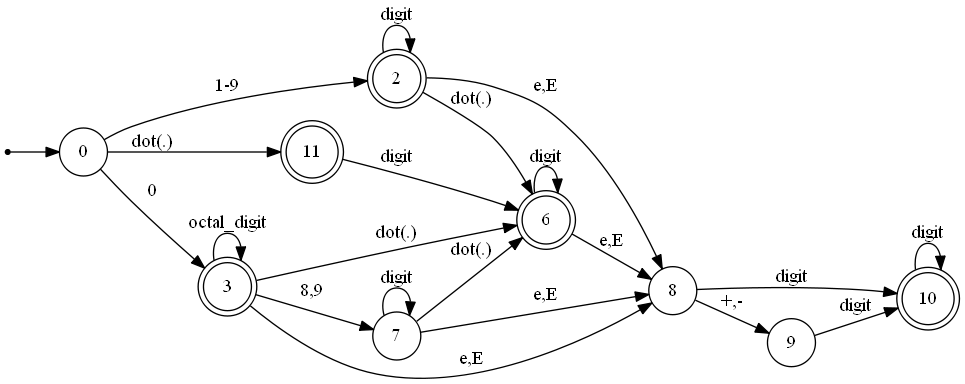
\includegraphics[width=\textwidth]{images/decimal_float.png}
	\caption{识别十进制浮点数的DFA}
	\label{fig:decimal_float}
\end{figure}

十六进制浮点数常量的定义如下所示。

\begin{lex}
hex-floating-constant:\\
	hex-prefix hex-fractional-constant binary-exponent-part \\
	hex-prefix hex-digit-sequence binary-exponent-part 
	
hex-fractional-constant:\\
	hex-digit-sequence . hex-digit-sequence \\
	hex-digit-sequence . \\
	. hex-digit-sequence
	
binary-exponent-part:\\
	bin-exp-flag digit-sequence \\
	bin-exp-flag sign digit-sequence
	
hex-digit-sequence:\\
	hex-digit \\
	hex-digit-sequence hex-digit
	
hex-prefix: \normalfont{one of}\\
{
	\normalfont
	\ttfamily
	0x 0X
}
\end{lex}

从定义中可以看出,十六进制浮点数必须有指数标志P,且指数部分的数字为十进制数。

转化为正规式如下所示。

\begin{lstlisting}
hex-float-constant = 
	0(x|X) hex-fractional-constant (p|P) (+|-)? digit+ (f|F|l|L)? |
	0(x|X) hex-digit+ (p|P) (+|-)? digit+ (f|F|l|L)?
hex-fractional-constant ->
	hex-digit+ . (hex-digit+)? |
	. hex-digit+
\end{lstlisting}

将其转化为等价的DFA如图\ref{fig:hex_float}所示。

\begin{figure}[htbp]
	\centering
	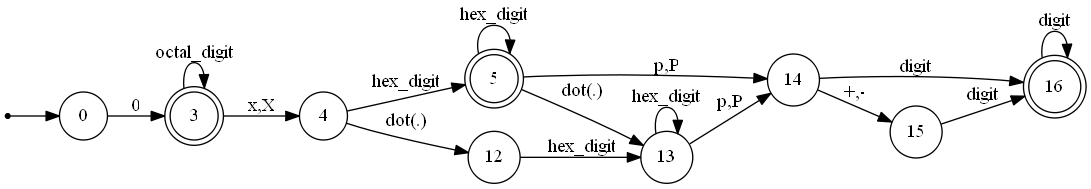
\includegraphics[width=\textwidth]{images/hex_float.png}
	\caption{识别十六进制浮点数的DFA}
	\label{fig:hex_float}
\end{figure}

\subsection{字符常量}
字符常量的词法定义如下所示。ISO C11标准中也定义多字节字符(multibyte character),即两个单引号之间允许有多个字符。本次实验中没有定义多字节字符。

\begin{lex}
character-constant:\\
	' c-char ' \\
	char-prefix ' c-char '
	
char-prefix: \normalfont{one of}\\
{
	\normalfont
	\ttfamily
	L u U
}

\itshape
c-char:\\
	any character except ', \, new-line \\
	escape-sequence
	
escape-sequence:\\
	simple-escape-sequence \\
	octal-escape-sequence \\
	hex-escape-sequence
	
simple-escape-sequence: \normalfont{one of}\\
{
	\normalfont
	\ttfamily
	$\backslash$' $\backslash$" $\backslash$? $\backslash\backslash$ $\backslash$a $\backslash$b $\backslash$f $\backslash$n $\backslash$r $\backslash$t $\backslash$v
}

\itshape
octal-escape-sequence:\\
	\ octal-digit \\
	\ octal-digit octal-digit \\
	\ octal-digit octal-digit octal-digit
	
hex-escape-sequence:\\
	\\x hex-digit \\
   hex-escape-sequence hex-digit
\end{lex}

字符常量整体上的定义非常简单,两个单引号之间包含一个字符。但从定义中可以看出,只是转义序列的处理比较麻烦。为了不因为细节而把核心问题淹没,先将只包含简单转义序列的词法转化为正规式,如下所示。

\begin{lstlisting}
character-constant = (L|u|U| ) ' normal-char | \ esc-char '
esc-char = '|"|?|a|b|f|n|r|t|v
\end{lstlisting}

等价的DFA如图\ref{fig:char}所示。其中接受态20就是真正的接受态,程序到达状态20后就可以直接识别为字符常量。

\begin{figure}[htbp]
	\centering
	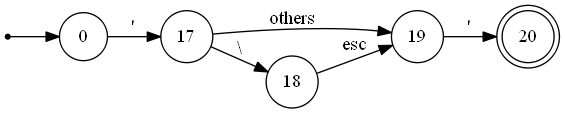
\includegraphics[scale=0.54]{images/char.png}
	\caption{识别基本字符常量的DFA}
	\label{fig:char}
\end{figure}

考虑八进制转义序列和十六进制转义序列的后的正规式如下所示。

\begin{lstlisting}
character-constant = (L|u|U| ) ' normal-char | \ esc-char | \ octal-digit (octal-digit octal-digit?)? | \x hex-digit+ '
esc-char = '|"|?|a|b|f|n|r|t|v
\end{lstlisting}

转化为等价的DFA如图\ref{fig:char2}所示。

\begin{figure}[htbp]
	\centering
	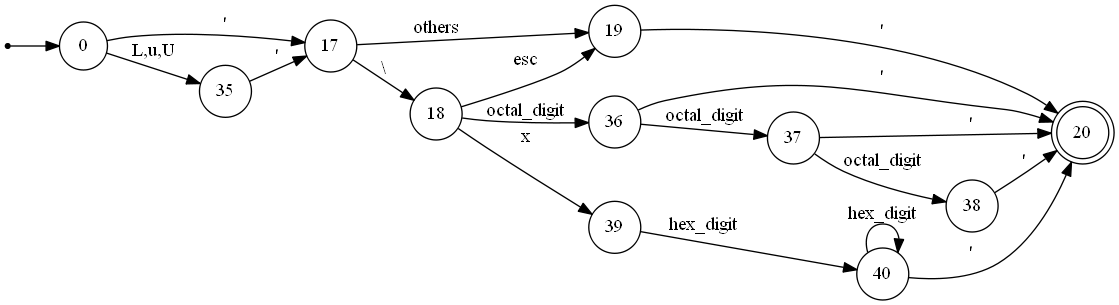
\includegraphics[width=\textwidth]{images/char2.png}
	\caption{识别完整字符常量的DFA}
	\label{fig:char2}
\end{figure}

\subsection{字符串}
字符串的词法定义如下所示。

\begin{lex}
string:\\
	" s-char-sequence "  \\
	encoding-prefix " s-char-sequence "
	
encoding-prefix: \normalfont{one of}\\
{
	\normalfont
	\ttfamily
	u8 u U L
}

\itshape
s-char-sequence:\\
	$\epsilon$  \\
	s-char-sequence s-char
	
s-char:\\
	any character except ", \\, new-line \\
	escape-sequence
\end{lex}

同字符常量,只考虑简单转义序列的正规式如下。

\begin{lstlisting}
string = u8|u|U|L|  " (normal-char | \ esc-char)* "
\end{lstlisting}

等价的DFA如图\ref{fig:string}所示。接受态23是真正的接受态,不需要读入额外的字符。

\begin{figure}[htbp]
	\centering
	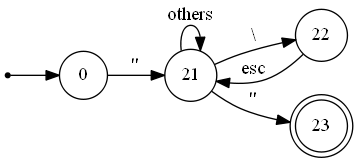
\includegraphics[scale=0.54]{images/string.png}
	\caption{识别基本字符串的DFA}
	\label{fig:string}
\end{figure}

考虑全部转义序列的正规式如下。

\begin{lstlisting}
string = u8|u|U|L|  " (normal-char | \ esc-char | \ octal-digit (octal-digit octal-digit?)? | \x hex-digit+)* "
\end{lstlisting}

将其转化为等价的DFA如图\ref{fig:string2}所示。因为实际的转换关系繁多,图中还是略去了一部分边,42、43、44和46状态,每个状态都省略了遇到普通字符回到21状态的边、遇到反斜线到22号状态的边和遇到非法字符到出错处理状态的边。

\begin{figure}[htbp]
	\centering
	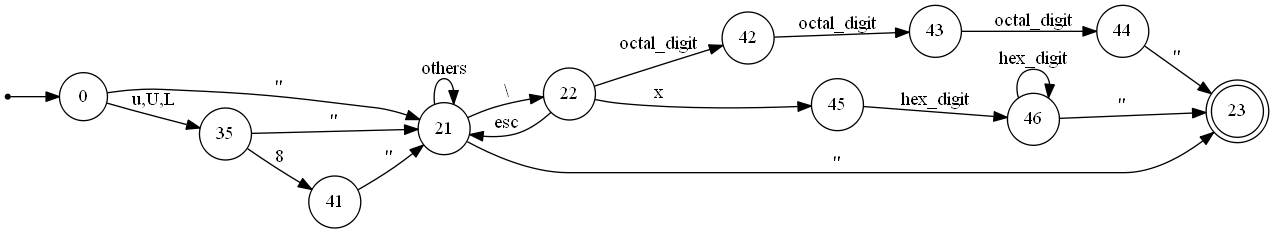
\includegraphics[width=\textwidth]{images/string2.png}
	\caption{识别字符串的DFA}
	\label{fig:string2}
\end{figure}

\subsection{分隔符}
将ISO C11中定义的分隔符分为限界符(delimiter)和运算符(operator)。如下所示。

\begin{lex}
delimiter: \normalfont{one of}\\
{
	\normalfont
	\ttfamily
	( ) [ ] \{ \} ; . ->
}

\itshape
operator: \normalfont{one of}\\
{
	\normalfont
	\ttfamily
	, ? : ~ \\
	+ += ++ - -= -- \& \&= \&\& | |= || \\
	< <= << <<= > >= >> >>= \\
	* *= / /= \% \%= \^ \^= ! != = ==
}
\end{lex}

限界符比较简单,基本上遇到限界符直接识别即可。而运算符比较复杂。根据第一个字符的区别将其分为以下几类。

\noindent
\textbf{\ttfamily ( ) [ ] \{ \} ; . ->}: 限界符。\\
\textbf{\ttfamily , ? : ~}: 这四个运算符不是任何运算符的前缀,遇到后直接识别即可。\\
\textbf{\ttfamily -}: 遇到-后可能是->限界符,也有可能是运算符。这是唯一一处限界符和运算符有交集的地方。\\
\textbf{\ttfamily + - \& |}: 这四个运算符的模式相同,可以单独作为运算符,也可以跟=,也可以自身重复一次。\\
\textbf{\ttfamily < >}: 可以单独作为运算符,可以跟=,可以重复自己,可以重复自己再跟等号=。\\
\textbf{\ttfamily * / \% \^ ! =}: 最普通的运算符。可以单独,也可以后跟等号=。\\

直接给出DFA如图\ref{fig:operator}所示。

\begin{figure}[htbp]
	\centering
	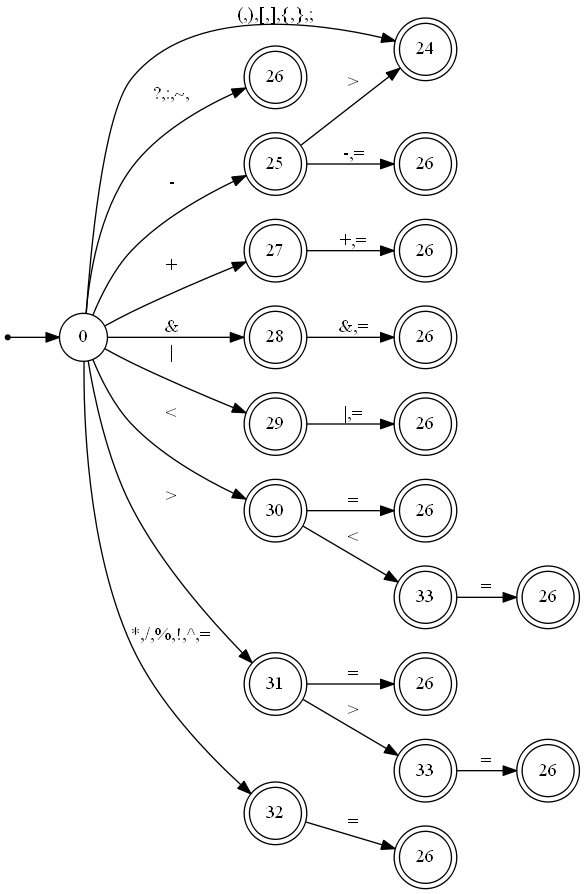
\includegraphics[scale=0.5]{images/operator.png}
	\caption{识别分隔符的DFA}
	\label{fig:operator}
\end{figure}

\subsection{出错处理}
出错处理也是词法分析过程中非常重要的一个部分,不可能编译的代码都是完全正确的,而一个好的出错处理机制可以准确地划分出不符合词法的部分,以保证代码的其他部分仍然能够正常识别,而出错处理设计不好时可能以为一处错误导致其他合法部分无法识别或将另外一些非法部分识别为合法。

实际上几乎自动机的每个状态节点要与出错处理机制相关联,因为几乎没有一个状态在接受任意字符后都有一个合法的后继状态定义,而对一个状态而言,接收到的所有合法字符之外的符号都是此状态的非法字符,都将转换到出错处理状态。

\begin{figure}[htbp]
	\centering
	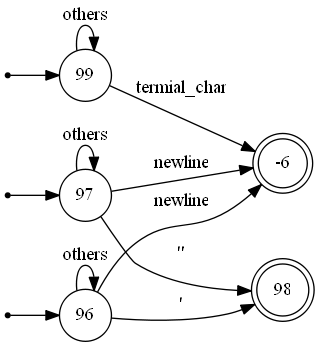
\includegraphics[scale=0.54]{images/error.png}
	\caption{负责出错处理的DFA}
	\label{fig:error}
\end{figure}

实验中与出错处理有关的状态定义了5个,如图\ref{fig:error}所示。一般情况下,遇到非法字符后将进入99状态,这个状态并不是接受状态,也就是遇到非法字符时并不会立即结束,而是继续读完整个非法单词,当遇到能够结束一个单词的符号,比如运算符或分隔符时,进入-6状态,识别非法单词结束,同时将这个终结符放回缓冲区,回到0状态开始新一轮的识别。

当在识别字符串时,也就是处理过双引号"后,遇到非法字符时进入97状态,不断接受字符知道字符串结束。非法字符串在两种情况下会结束,遇到回车换行符时进入-6状态,识别非法字符串,将回车换行符放回缓冲区,重新开始新一轮识别;遇到双引号"时,进入98状态,立即结束识别,双引号作为非法字符串的最后一个字符被识别,不再送回缓冲区。类似的,在识别字符常量时遇到非法字符将进入96状态,遇到单引号或回车换行符时结束识别。

\subsection{最终DFA}
将前文所有设计的DFA合并到一起称为最终的DFA,如图\ref{fig:dfa}所示。介于绘图中节点布局的因素,部分状态和边没有画出,包括整数和浮点数常量的后缀识别,字符常量和字符串的八进制转义序列和十六进制转义序列的识别,每个节点的出错处理部分和程序中真正的接受状态。但在实际程序中全部实现了。每个状态的编号已经事先调整好了,上文中分部分介绍中的编号就是最终合并调整后的编号,没有编号冲突。

\begin{figure}[htbp]
	\centering
	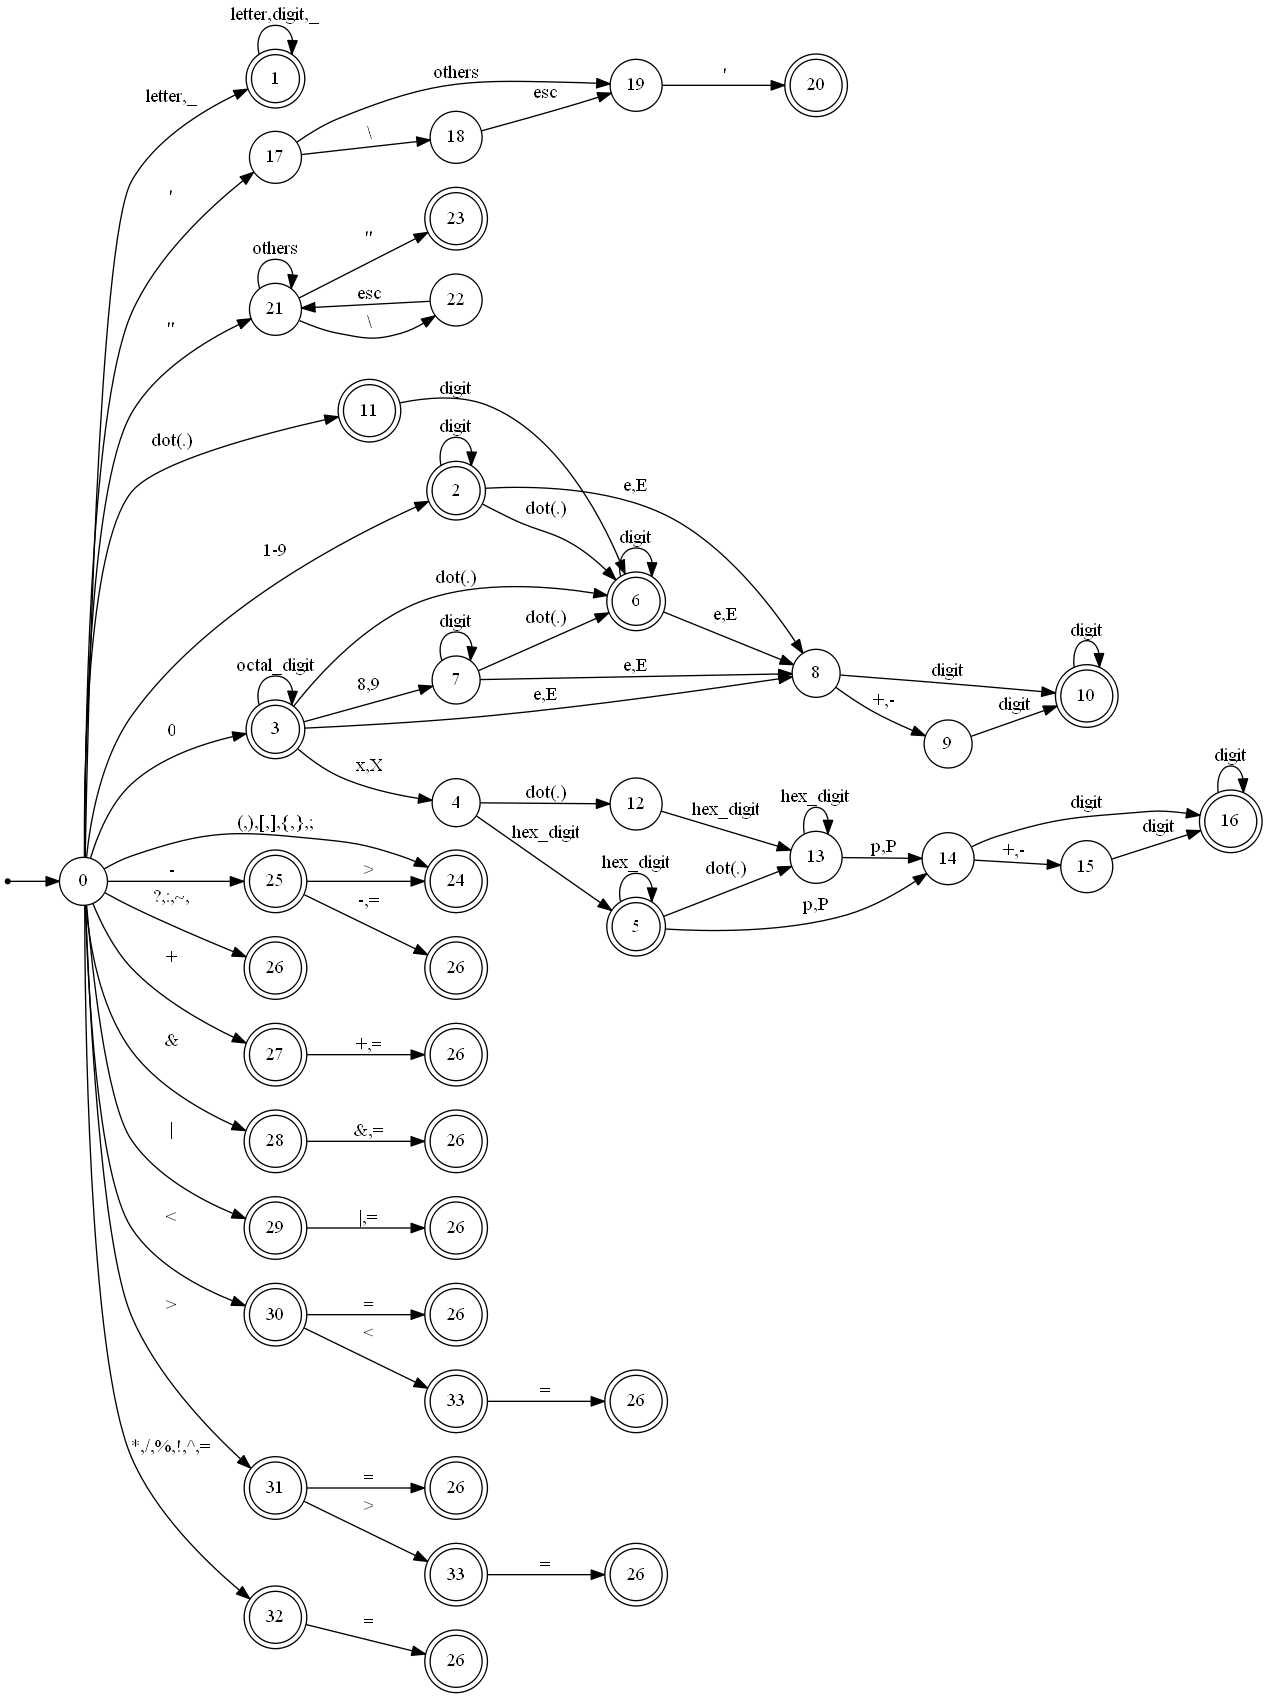
\includegraphics[width=\textwidth]{images/dfa.png}
	\caption{合并后的DFA}
	\label{fig:dfa}
\end{figure}

\subsection{程序实现}
程序使用Java语言实现,使用以程序为中心的方法,对自动机中的每个状态都定义一个转换函数,以确定当前状态接收不同字符后的后继状态。主程序的伪代码如下。其中输入缓冲区为buffer,buffer.next()表示从缓冲区读取一个字符,buffer.push(c)表示将字符c放回缓冲区。接受状态集合为Accept,其中有一些接受状态是读取了一个额外字符后才识别单词的,处理这些状态时需要向缓冲区中放回一个字符,这些状态包含在回退接受态集合Back中。

\begin{algorithm}[H]
\begin{multicols}{2}
	\caption{Scanner}
	\begin{algorithmic}[1]
		\REQUIRE ~\\
			输入缓冲区buffer\\
			接受状态集$Accept$\\
			回退接受状态集$Back$
		\ENSURE ~\\
			属性字流$(type_i, word_i)$
		\STATE 状态$state \leftarrow 0$
		\STATE 当前单词$word \leftarrow \{\}$
		\STATE $c \leftarrow$ buffer.next()
		\WHILE{$c \neq$ EOF}
			\STATE $word$ += $c$
			\STATE $f \leftarrow$ 状态$state$的转换函数
			\STATE $state \leftarrow f(c)$
			\IF{$state \in Accept$}
				\IF{$state \in Back$}
					\STATE buffer.push(c)
					\STATE $word$ -= $c$
				\ENDIF
				\STATE $type \leftarrow attr(state)$
				\STATE output $(type_i, word_i)$
				\STATE $state \leftarrow 0$
				\STATE $word \leftarrow \{\}$
			\ENDIF
			\STATE $c \leftarrow$ buffer.next()
		\ENDWHILE
	\end{algorithmic}
	\end{multicols}
\end{algorithm}

核心的Java实现代码如下所示。每一个状态的转换函数名为“state+状态序号”,程序中的getMethod()和invoke()函数是Java中的反射技术,根据当前的状态值动态地获取对应的状态转换函数来执行。

\begin{lstlisting}[language=Java]
public void run(String inputFile, String outputFile) {
	// Build buffer "reader" from "inputFile"
	int state = 0;
	StringBuilder word = new StringBuilder();
	Class<?> cl = this.getClass();
	for (int r = reader.read(); r != -1; r = reader.read()) {
		char c = (char)r;
		word.append(c);
		Method action = cl.getMethod("state" + state, char.class);
		state = (int) action.invoke(null, c);
		if (isAcceptState(state)) {
			if (isBackState(state)) {
				reader.unread(c);
				word.setLength(word.length() - 1);
			}
			dealAcceptState(state, word.toString());
			word.setLength(0);
			state = 0;
		}
	}
  	// Write to "outpuFile"	
}
\end{lstlisting}

\section{实验结果}
src文件夹中又三个Java源程序文件,分别实现了三个Java类,BITMiniCC、MiniCCPreProcesser和Scanner。

其中BITMinicCC是主类,是编译器的框架,里面我将原有的框架做了一些修改,但对外的特性完全没有变,修改的具体内容在报告的最后一部分给予了说明。

MiniCCPreProcesser是对框架附带的预处理jar包中的class文件反编译后的结果,并作了稍许修改。因为时间的原因,我没有自己实现预处理器。但是框架自带的预处理器功能不完整,而且bug颇多,我先临时借来使用,以保证程序流程完整执行。但也可以直接拿预处理过的文件或者不带预处理内容的文件进行词法分析测试。

Scanner是词法分析器,所有的词法分析功能在Scanner类中实现。Scanner中定义了main方法,可以单独运行,单独运行时需要在命令行中给出要处理的文件名。同时Scanner也定义了run方法,供BITMiniCC框架调用。单独使用Scanner时,在生成单词属性流XML文件的同时,在控制台中也会以简洁的方式打印识别出的每个单词的行号,内容和属性,便于查看。当使用框架调用时,不会在控制台输出属性流内容。

向词法分析器输入预处理后的C语言代码如下所示。

\begin{lstlisting}[language=C]
int main()
{
	printf("Hello\n");
	int a = 1 + 012 * 0xf5;
	double b=++a*0x/08.2E-3;
	char *p = "\12\xff"
	return 0;
}
\end{lstlisting}

输出的属性字流如下所示。程序最终将其转换为规定的XML文件保存。

\begin{multicols}{2}
\begin{lstlisting}[xleftmargin=1cm,xrightmargin=1cm]
int       keyword
main      identifier
(         delimiter
)         delimiter
{         delimiter
printf    identifier
(         delimiter
"Hello\n" string
)         delimiter
;         delimiter
int       keyword
a         identifier
=         operator
1         constant
+         operator
012       constant
*         operator
0xf5      constant
;         delimiter
double    keyword
b         identifier
=         operator
++        operator
a         identifier
*         operator
0x        illegal
/         operator
08.2E-3   constant
;         delimiter
char      keyword
*         operator
p         identifier
=         operator
"\12\xff" string
return    keyword
0         constant
;         delimiter
}         delimiter
\end{lstlisting}
\end{multicols}

国际C语言混乱代码大赛(IOCCC)2013年的获奖作品misaka的代码如图\ref{fig:misaka-c}所示。

\begin{figure}[htbp]
	\centering
	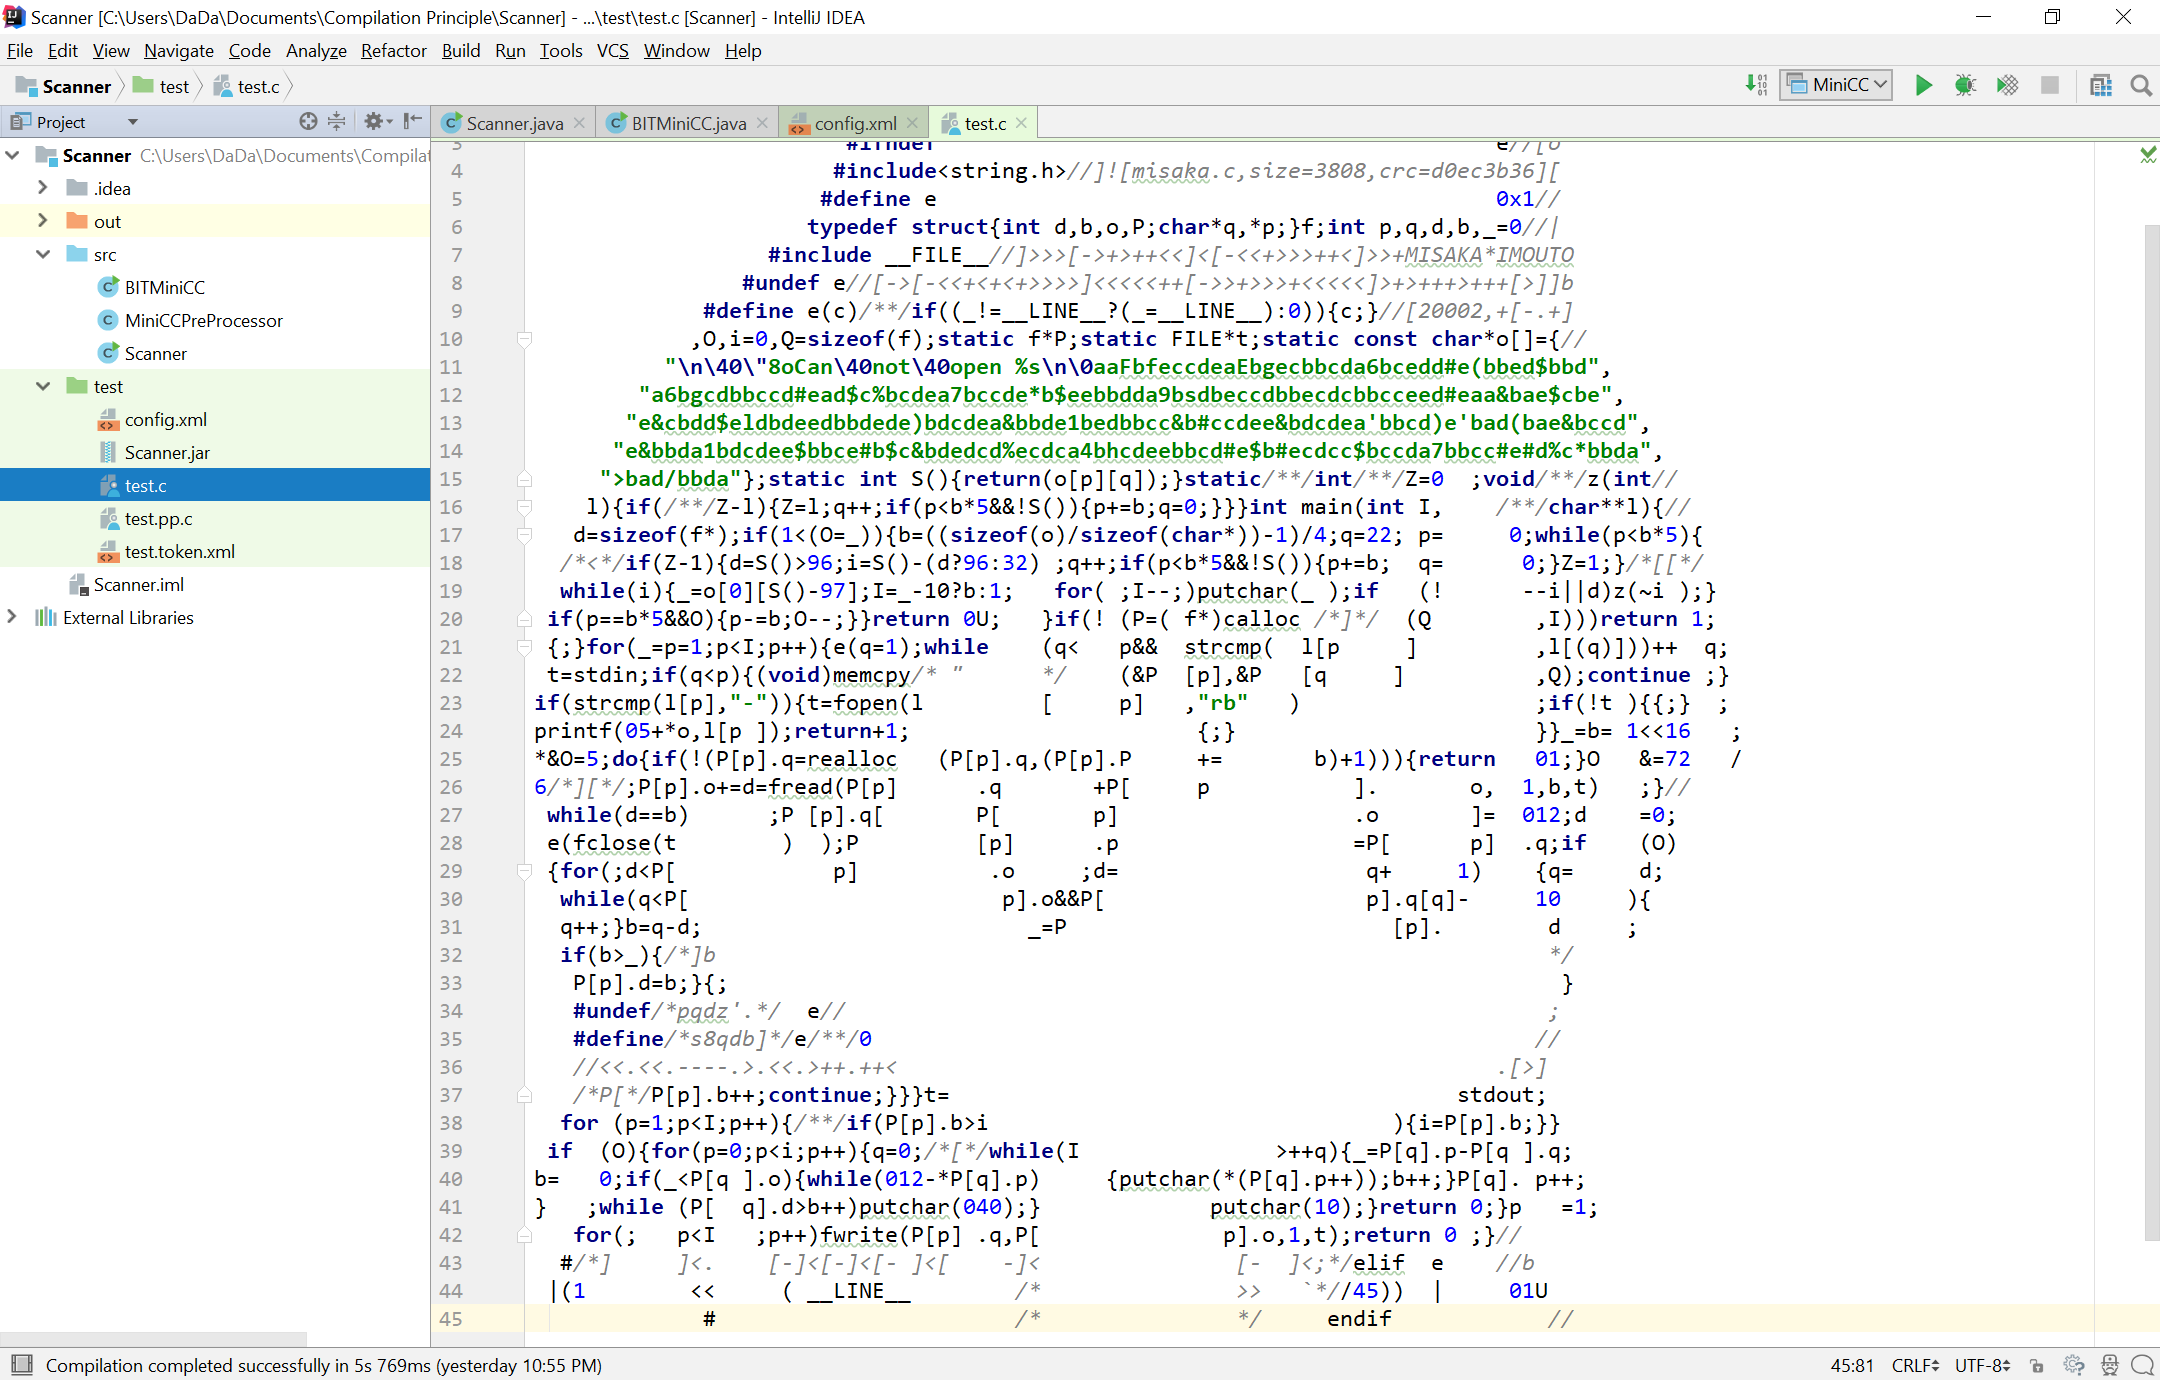
\includegraphics[width=0.97\textwidth]{images/misaka-c.png}
	\caption{misaka.c源文件}
	\label{fig:misaka-c}
\end{figure}

将其预处理后输入词法分析其,得到的包含属性字流的XML文件如图\ref{fig:misaka-token}所示。

\begin{figure}[htbp]
	\centering
	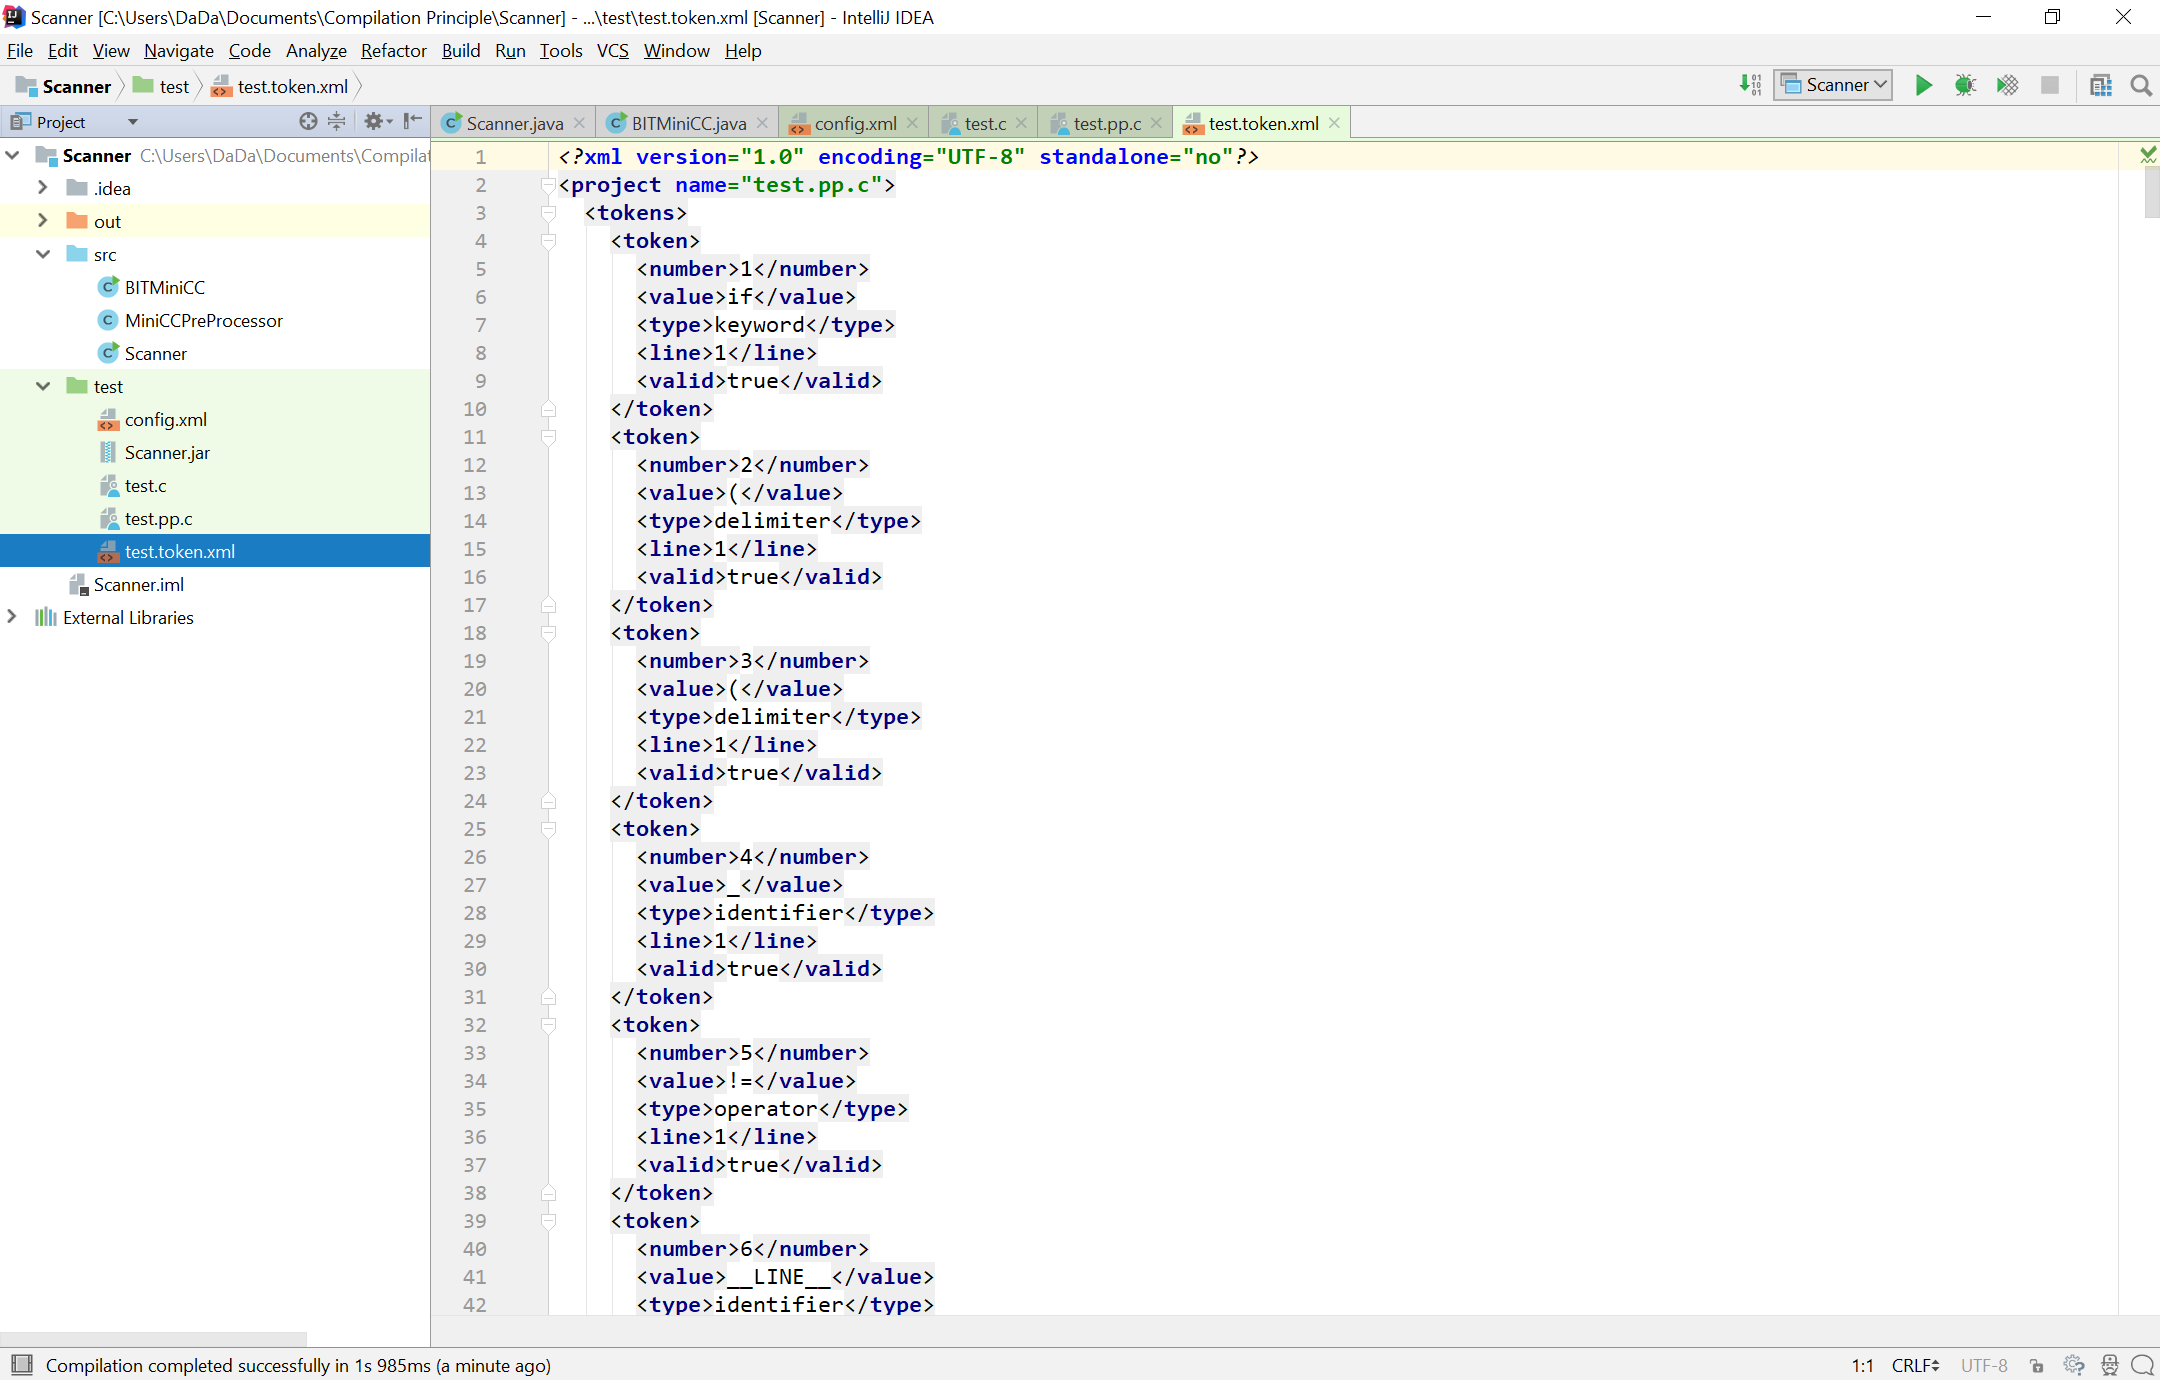
\includegraphics[width=0.97\textwidth]{images/misaka-token.png}
	\caption{词法分析后的misaka.token.xml文件}
	\label{fig:misaka-token}
\end{figure}

\section{心得体会}
通过本次实验,我基本掌握了词法分析的基本知识,在有限自动机的设计和简化上有了很多的练习,并且在代码实现的过程中,进一步提高了对Java语言的理解和熟练度。通过使用老师提供给我们的编译器框架,我非常清晰地看到了一个编译器的组成,并且更加熟悉了一个代码在从我们平日里点击“编译”之后,整个编译流程所需要进行的各个步骤。

在实验中感触最深的就是,在设计有限自动机的时候,由于之前设计大型DFA、NFA比较少,导致在遇到较为复杂的情况时,比如遇到浮点数识别或者转义字符识别时,需要反复修改NFA,逐渐学习掌握消除无关状态和等价状态的相关方法的用法。

次外也切实体会到了Java语言面向对象设计的强大,可以为开发大型工程时提供极大的便利。

\section{框架修改}
原有的BITMiniCC框架的代码有些过于冗长,其实现的功能非常简单,只是根据配置文件config.xml中的内容依次调用编译各阶段的程序,将上一个程序的输出文件作为当前程序的输入文件,仅此而已。而原有的框架把这种只需要循环就可以完成的工作复制粘贴了好几份,顿时使得本来简单的代码变得过于冗长、难于阅读和难于修改。我将原代码中功能相同的代码合并到了一个循环中,并优化了部分部分代码的写法,同时完全兼容原有的config.xml中的配置,希望可以对老师今后的教学活动有所帮助,也希望能帮助其他同学更好更快地理解和使用框架。

此外,我对老师提供的配置文件config.xml的格式也有一个小建议。文件的根元素是一个config标签,核心信息是对应8个阶段的phase标签,但是根标签与核心标签之间却套了两层额外的标签phases和phase,如下所示。这两层额外的框架标签给阅读和解析文件的内容增加了负担,而且外层的phase标签与核心的phase标签重名,更是给解析过程带来了混乱,也不利于文件框架的清晰定义。所以,我建议老师去掉中间的两层phases和phase标签。

\begin{lstlisting}[language=XML]
<?xml version="1.0" encoding="UTF-8"?>
<config name="config.xml">
  <phases>
    <phase>
      <phase skip="false" type="java" path="" name="pp" />
      <phase skip="false" type="java" path="" name="scanning"/>
      ...
\end{lstlisting}

再者,原有框架中将编译过程每一步的输入文件输出文件后缀名在代码中固定了,同学们必须严格按照规定的后缀名给文件命名,并且如果不阅读源代码往往不容易明确得到这些文件名的定义,这也给同学们理解和使用框架带来了一定的阻力,并且破坏了设计框架的初衷,方便同学,为同学们搭建完整编译器提供帮助,而不是再给同学们出一道阅读代码的题目。所以,我建议在每一个核心phase标签上再加一个属性,用来让同学们指定自己的文件后缀名,当然,老师可以提供默认的建议后缀名。

最后一个建议,整个框架中程序间信息的交换完全基于XML格式文件,鉴于XML格式文件有繁多的标签属性,信息密度并不大,且可阅读性还是稍微差一些,而且同学们要完成整个编译器不得不学习XML文件的读取和创建的技术,这无形中又给同学们增加了额外的并不在教学目标中的负担。老师可以考虑一下近来非常流行,也非常轻量级且更易于阅读和自动化处理的json格式的文件,功能于XML完全相同,但更加方便。比如配置文件可以是这样。

\begin{lstlisting}[language=Java,
	xleftmargin=1cm,xrightmargin=1cm]
{
  "phases": [
    {
      "skip": false,
      "type": "java",
      "path": "",
      "name": "pp",
      "suffix": ".pp.c"
    },
    {
      "skip": false,
      "type": "java",
      "path": "",
      "name": "scanning",
      "suffix": ".token.json"
    },
    ...
  ]
}
\end{lstlisting}

词法分析器输出的单词属性流可以是这样。

\begin{lstlisting}[language=Java,
	xleftmargin=1cm,xrightmargin=1cm]
{
  "tokens": [
    {
      "number": 1,
      "value": "int",
      "type": "keyword",
      "line": 1,
      "valid": true
    },
    {
      "number": 2,
      "value": "main",
      "type": "identifier",
      "line": 1,
      "valid": true
    },
    ...
  ]
}
\end{lstlisting}

把多年来的XML文件替换为json文件可能会涉及很多地方的修改,并且由于思维惯性的原因,突然改变的难度很大,我也是仅此向老师说出我的想法,希望我们的BITMiniCC框架能越来越好,成为北理工编译原理课程代表性的一个特色。

\cleardoublepage

\newpage\null
\thispagestyle{empty}
\cleardoublepage

\end{document}





















